\documentclass[a4paper, 12pt]{article}

% LaTeX файл с преамбулой не должен содержать команду documentclass и \begin{document}. Эти команды должны находиться только в основном документе!

\usepackage[english, russian]{babel}
\usepackage[T2A]{fontenc}
\usepackage[utf8]{inputenc}

\tikzset{help lines/.style = {very thin, gray}} % Задание стиля вспомогательных линий (; не нужна (!))

\begin{document}
    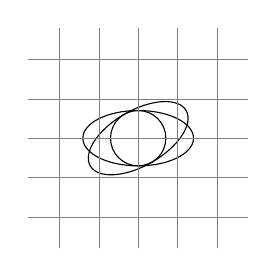
\begin{tikzpicture}
        \draw (0, 0) circle (10pt); % Круг
        \draw (0, 0) ellipse (20pt and 10pt); % Эллипс
        \draw [rotate = 30] (0, 0) ellipse (20pt and 10pt); % Повёрнутый эллипс

        \draw [step = .5cm, gray, very thin] (-1.4, -1.4) grid (1.4, 1.4);
        % step = .5cm <=> step = 0.5cm (с нулём понятнее запись);
        % gray - цвет линий сетки (серый);
        % very thin - толщина линий сетки (очень тонкие).

        % Или
        % \tikzset{help lines/.style = {very thin, gray}} <-- (можно здесь, но лучше в файле преамбулы или перед \begin{document})
        % ^^^ Задание стиля вспомогательных линий (; не нужна (!))
        \draw [step = .5cm, help lines] (-1.4, -1.4) grid (1.4, 1.4);
    \end{tikzpicture}
\end{document}